\documentclass[a4paper]{article}

\usepackage[T1]{fontenc}
\usepackage[utf8x]{inputenc}
\usepackage[a4paper]{geometry}
\geometry{verbose,tmargin=2cm,bmargin=2cm,lmargin=1cm,rmargin=1cm,headheight=1cm,headsep=1cm,footskip=1cm}
\usepackage{fancyhdr}
\pagestyle{fancy}
\setlength{\parskip}{\medskipamount}
\setlength{\parindent}{0pt}
\usepackage{graphicx}

\makeatletter
\usepackage{lastpage}
\usepackage{indentfirst}
\usepackage{mathrsfs}

\lhead[lh-even]{Edgar Vedvik\\ Informatikk}
\chead[ch-even]{TDT4145 Datamodellering og databasesystemer\\ Øving 1}
\rhead[rh-even]{\today}

\lfoot[lf-even]{}
\cfoot[cf-even]{Side \thepage{} av \pageref{LastPage}}
\rfoot[rf-even]{}

\date{}

\makeatother

\usepackage[english]{babel}

\begin{document}
\thispagestyle{fancy}

\subsection*{1a.}

Data er informasjon om noe som er lagret. En database er en strukturert samling av data. Et databasesystem er samlingen av en database og programvaren som kjører databasen (databasemotoren)

\subsection*{1b.}

I en database er det bestemte regler for hvordan man kan hente ut og legge til data. Programvaren kan da hente ut og legge til data med denne strukturen. Tradisjonelle filsystemer lagrer data på mange forskjellige måter, og programvaren må vite hvordan den skal hente ut denne dataen.


\subsection*{1c.}

Fordelene med databasesystemer er struktur, raskere tilgjengelighet og bedre søkbarhet.

\subsection*{2.}

\noindent
\begin{center}
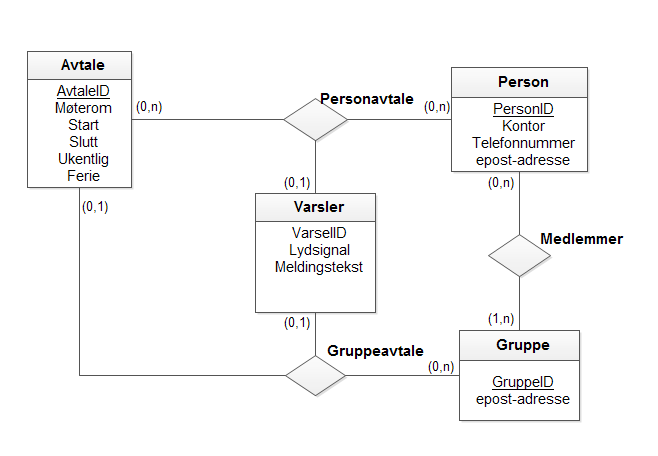
\includegraphics[width=0.8\textwidth]{oving1-2.png}
\par\end{center}

\subsection*{3.}

\begin{center}
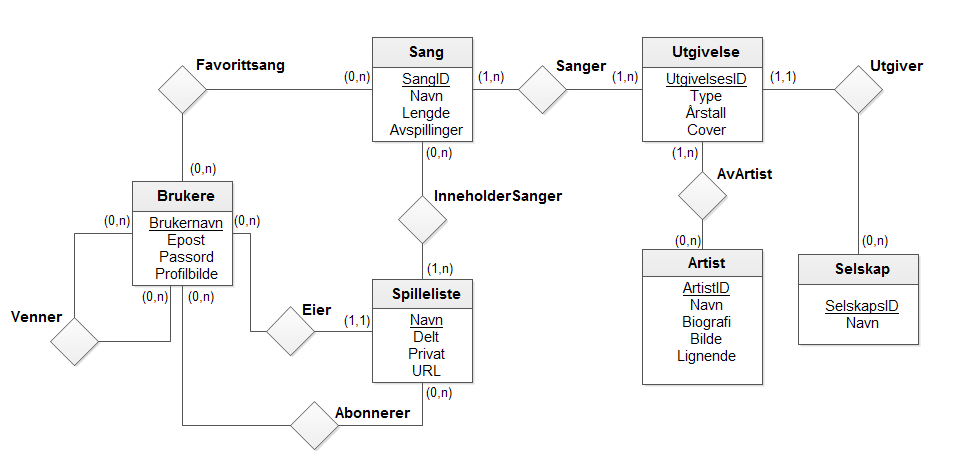
\includegraphics[width=1\textwidth]{oving1-3.png}
\par\end{center}

\subsection*{4.}

\begin{center}
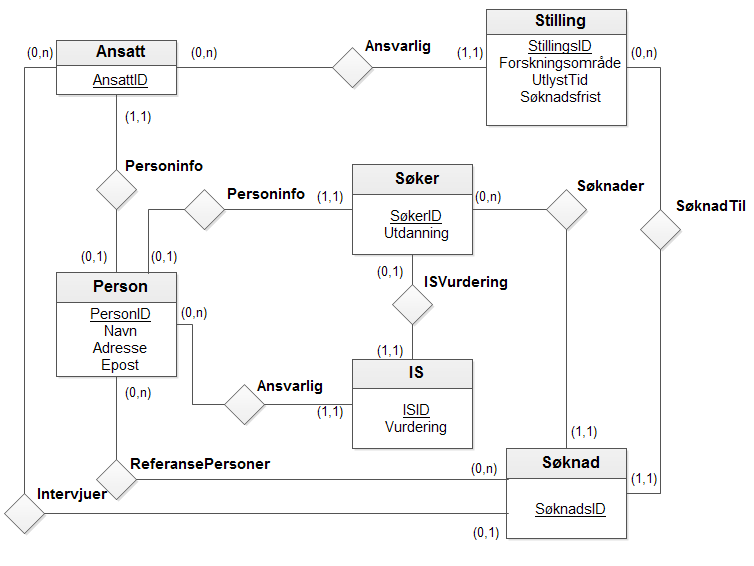
\includegraphics[width=0.9\textwidth]{oving1-4.png}
\par\end{center}

\end{document}